\documentclass{article}

\usepackage[english]{babel}
\usepackage[utf8]{inputenc}
\usepackage{amsmath,amssymb}
\usepackage{parskip}
\usepackage{graphicx}
\usepackage{subcaption}
\graphicspath{{figures/}}

\usepackage[obeyspaces]{url}

\usepackage{booktabs} \usepackage{siunitx}

\usepackage{hyperref}
\hypersetup{
    % colorlinks = true,
    linkcolor = blue,
    filecolor = magenta,
    urlcolor = cyan,
    pdftitle = {Assignment 2 for DGP 486},
    pdfpagemode = FullScreen,
}

\usepackage{natbib}
\bibliographystyle{abbrvnat}
\setcitestyle{authoryear,open = {(},close = {)}}


\usepackage[top = 2.5cm, left = 3cm, right = 3cm, bottom = 4.0cm]{geometry}
\usepackage[table]{xcolor}

\newcommand{\tablespace}{\\
[1.25mm]}
\newcommand\Tstrut{\rule{0pt}{2.6ex}} \newcommand\tstrut{\rule{0pt}{2.0ex}} \newcommand\Bstrut{\rule[-0.9ex]{0pt}{0pt}}
\title{Assignment 2 for DGP 486}
\author{Yangyang Li\\
 yangyang.li@northwestern.edu}
\date{\today}

\begin{document}

\maketitle

\section{Part 1}

\textbf{Use one paragraph to describe the biological system in your project and explain the goal of identifying epigenomic differences}

Spatial organization of the genome plays a central role in gene expression.
But current epigenomic approaches largely map DNA regulatory elements outside of the native context of the nucleus.
The paper develop transposase-accessible chromatin with visualization (ATAC-see)~\citep{Chen2016}.
A central question in epigenetics is how chromatin organization is disassembled and reassembled during the cell cycle.
The paper employed ATAC-see and DAPI staining of DNA content for fluorescence activated cell sorting (FACS) in human B-cell line GM12878.
There are two groups of cells G1-low and G1-high.
G1-low sample means it has a lower level of ATAC-see signal.
G1-high sample means it has a high level of ATAC-see signal
The paper regard G1-low as control and G1-high as treatment.


\textbf{Process the ATAC-seq data and report mapping statistics}

I use fastq~\citep{Chen2018} to trim and profile the ATAC-seq data (Figure~\ref{fig:ms}).

\begin{figure}[h]

	\begin{subfigure}
		{0.5\textwidth}
		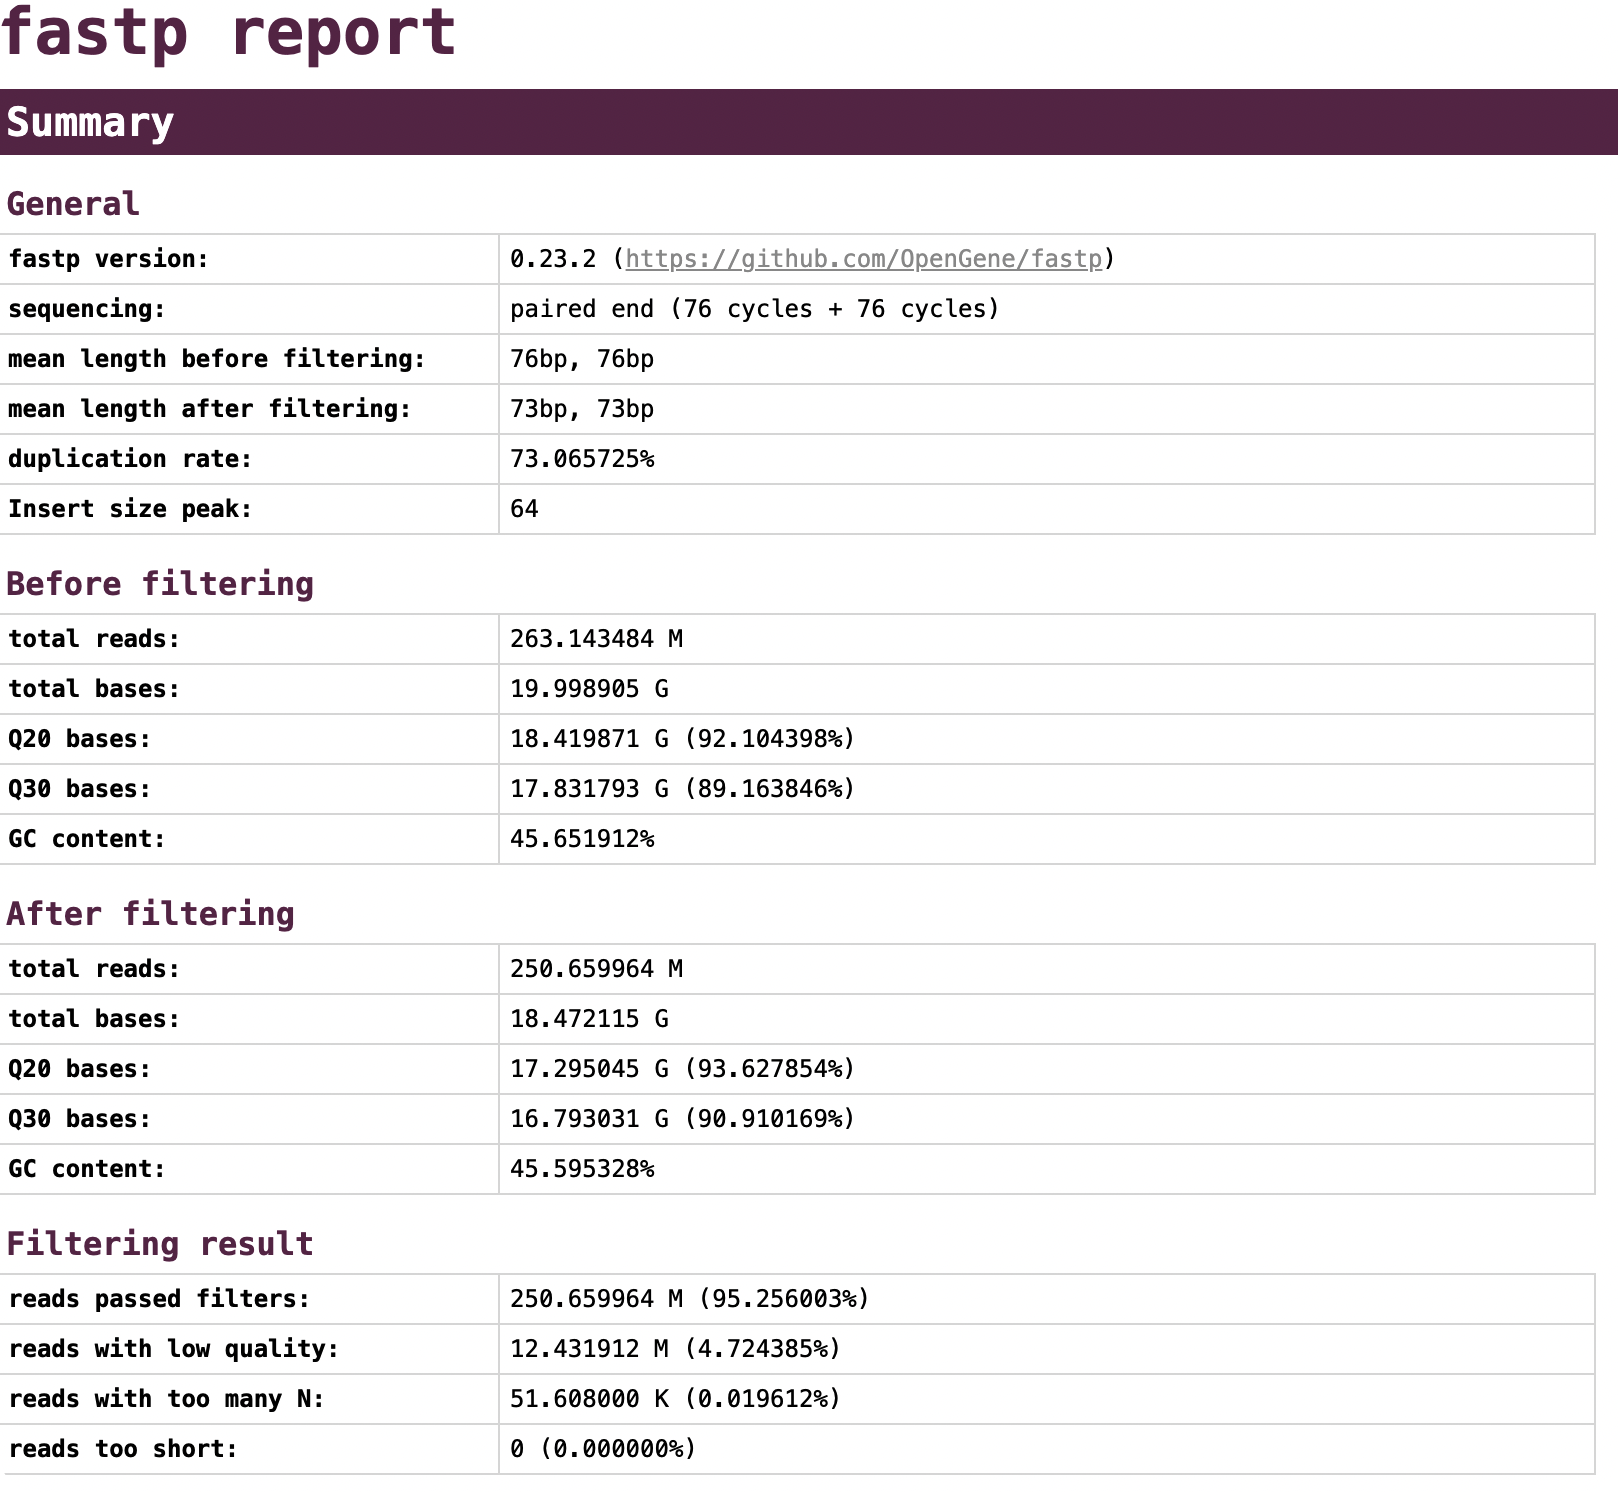
\includegraphics[width = 1.5\linewidth ]{high-qc.png}
		\caption{G1-high}
		\label{fig:g1-high-qc}


	\end{subfigure}



	\begin{subfigure}
		{0.5\textwidth}
		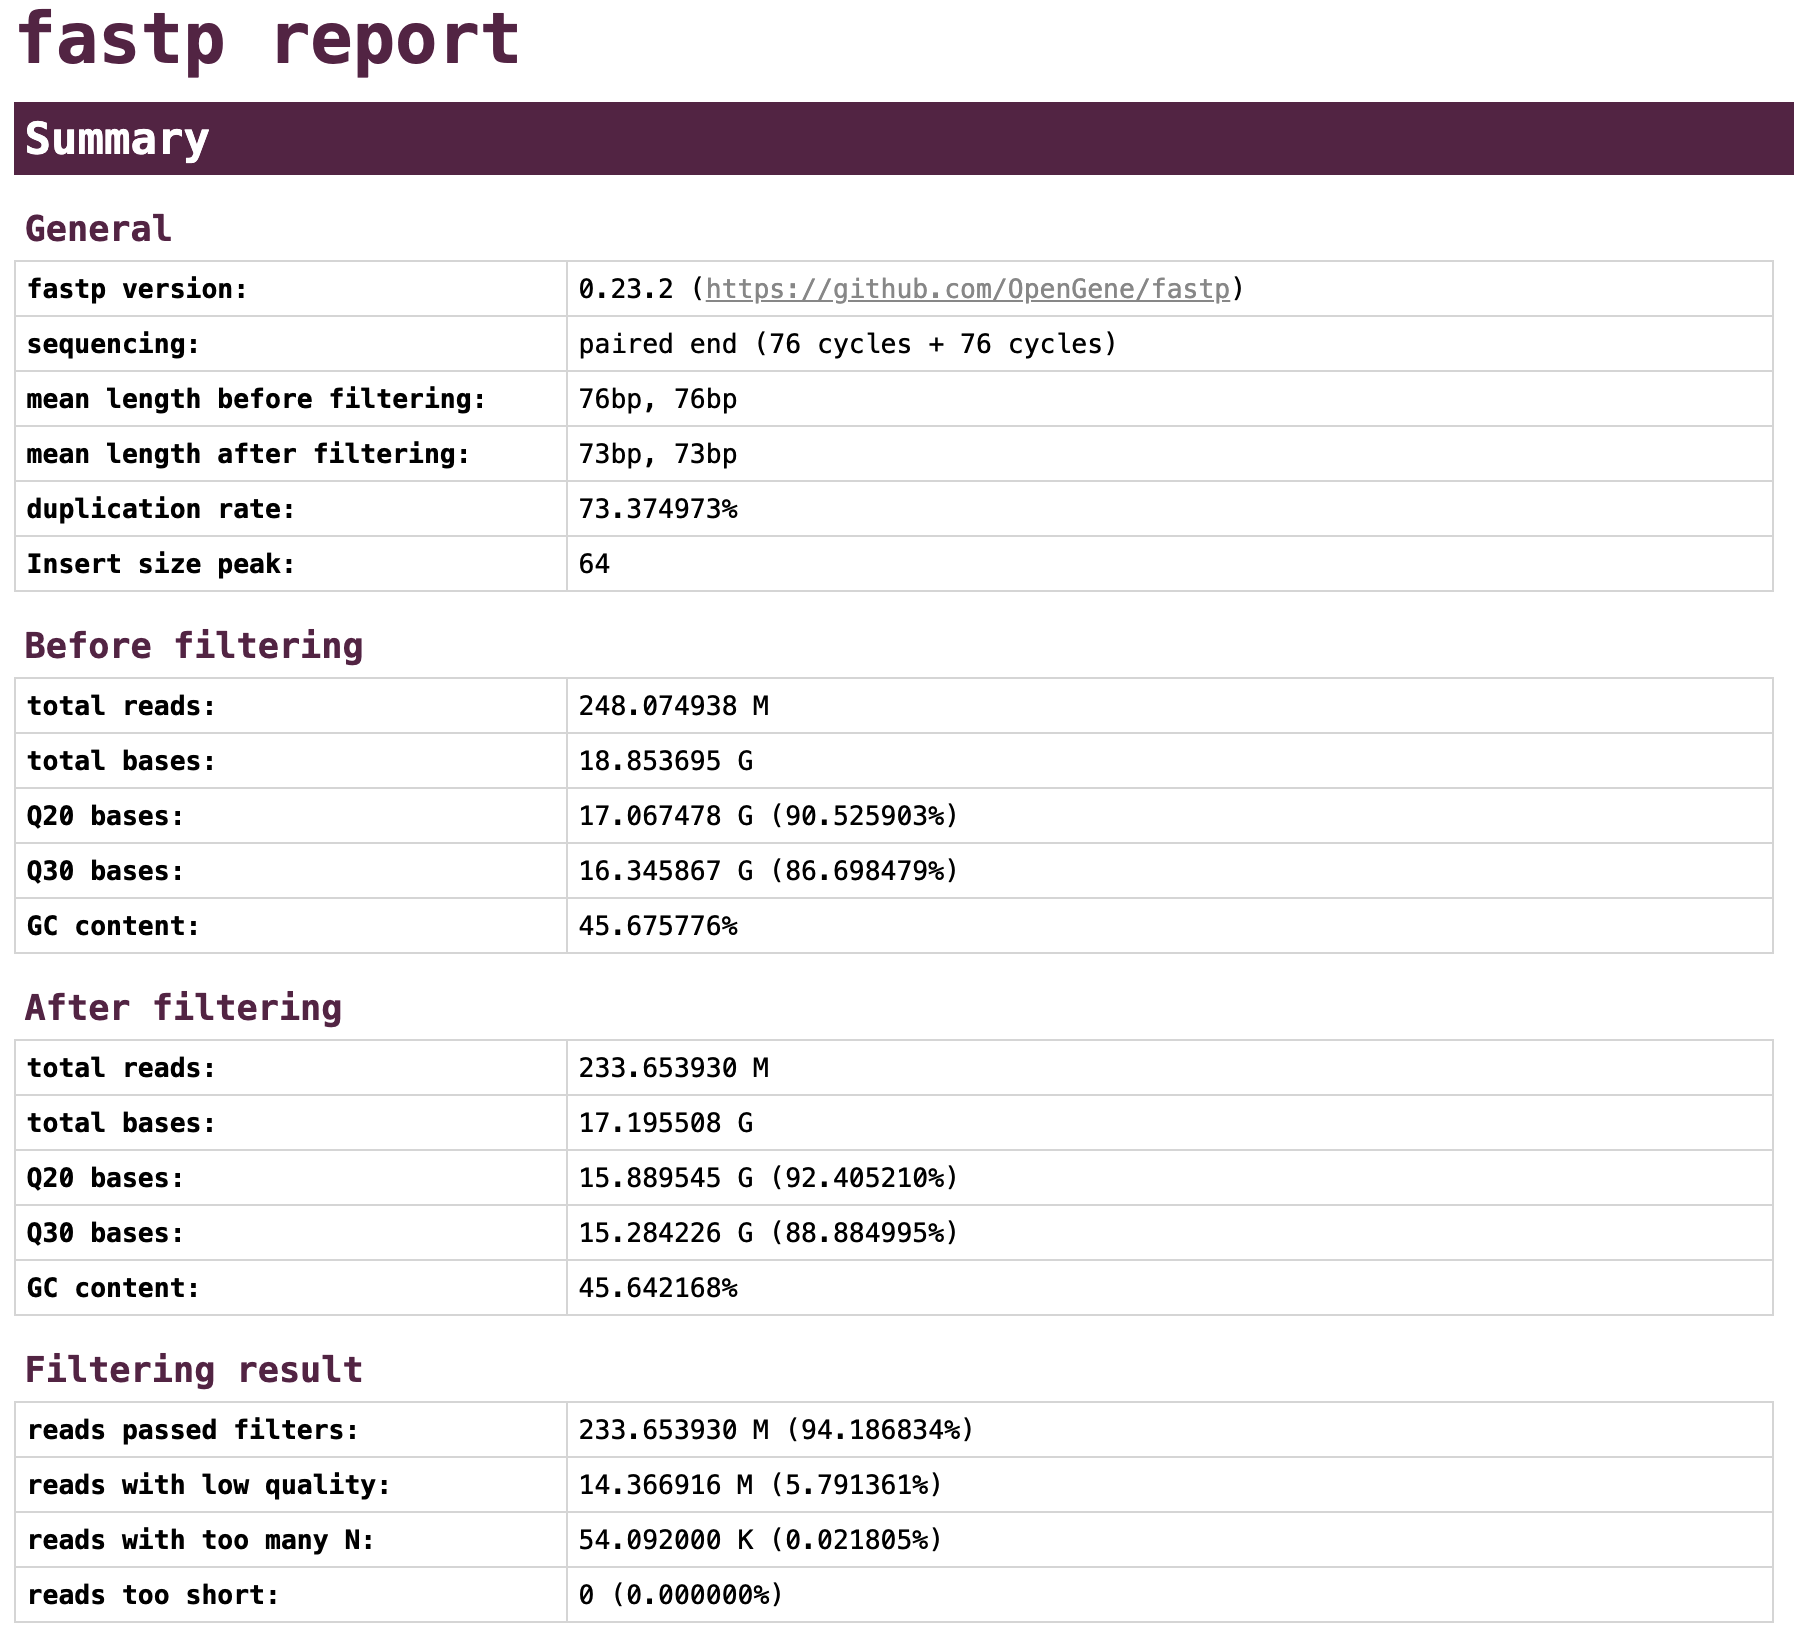
\includegraphics[width = 1.5\linewidth ]{low-qc.png}
		\caption{G1-low}
		\label{fig:g1-low-qc}


	\end{subfigure}

	\caption{Mapping Statistics}
	\label{fig:ms}
\end{figure}


\textbf{Identify tissue-specific or condition-specific ATAC-Seq peaks}


There exists some condition-specific ATAC-Seq peaks in G1-high sample.
For example, \textit{chr1-228174127-228174497} and \textit{chr2-115438873-115439201}.
The result is located at \path{/projects/e31900/yangyangli/data/assignment2/atac-seq/atac_peaks.narrowPeak.bed}

\textbf{Draw heatmap for the condition-specific ATAC-Seq peaks}

Figure~\ref{fig:heat} shows the heatmap of G1-high sample.

\begin{figure}
	\centering
	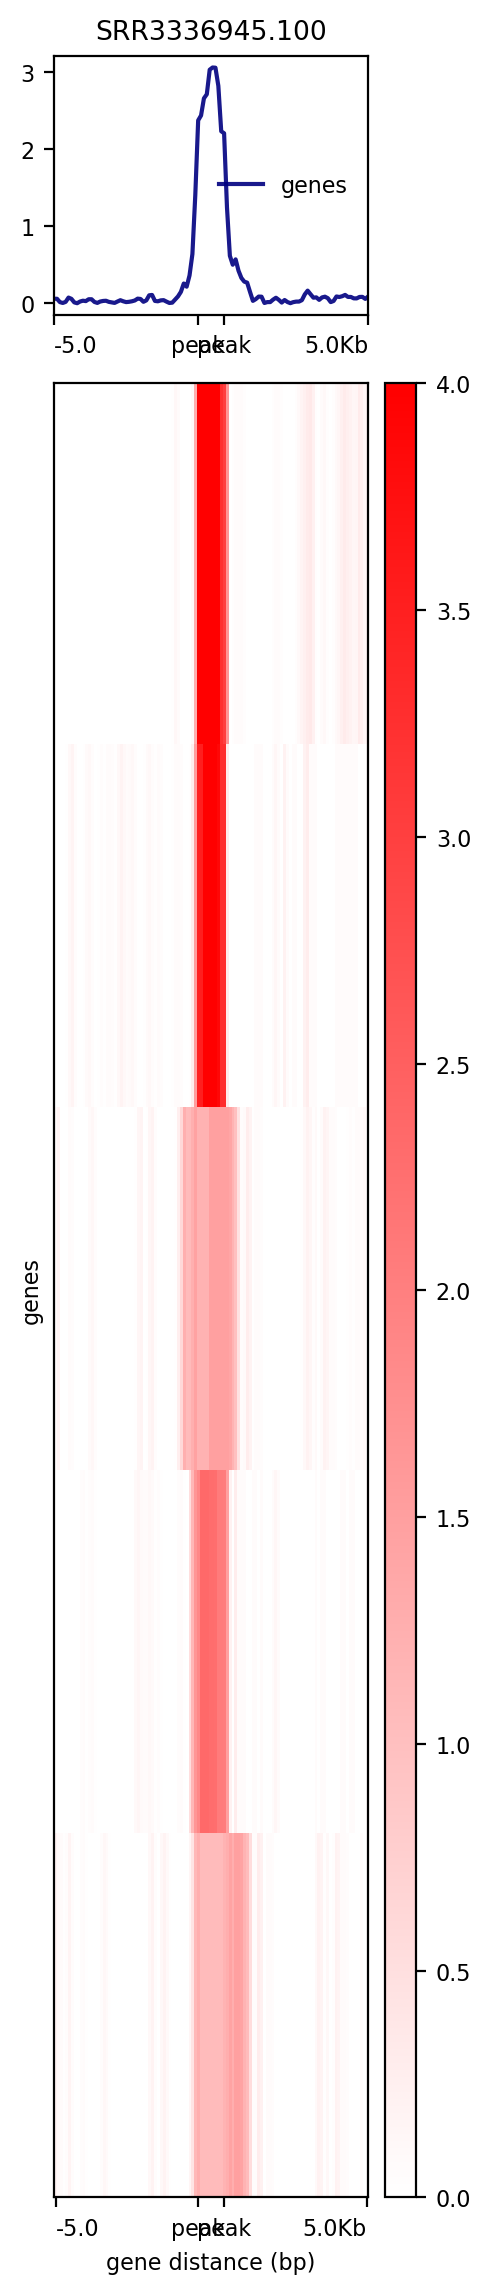
\includegraphics[scale = 0.8]{atac.peak.heatmap.png}
	\caption{Heatmap}
	\label{fig:heat}
\end{figure}


\textbf{Perform motif search in tissue/condition-specific open chromatin regions and report the top five motifs}

Unfortunately, I did not find the condition-specific regions and motifs due to the experiments design~\citep{Chen2016}.
The paper does not follow traditional analysis pipeline.
They want to use ATAC-seq to verify their new method.
However, the intermediate results are located at \path{/projects/e31900/yangyangli/data/assignment2/atac-seq}.


\textbf{Use one paragraph to explain whether the TFs identified in the condition-specific regions are relevant to the condition}

The region \textit{chr6-601378-602031} is an interesting region and the region cover two peaks
The region is related to H3K27Ac Mark that often found near regulatory elements.


\textbf{Pick one TF from each condition and the claims needs to be support by current literature}

The experiments design in the paper does not contain analysis of TF.
Hence, I did not find some interesting finding about TF.
However, The paper found that gene ontology analysis showed that the accessible elements in G1-high cells were enriched for genes with histone acetyltransferase activity, histone modification, gene transcription, nuclear body and other biological process \citep{Chen2016}.

\textbf{Summary}

I use Snakemake, which can ensure the reproducibility, to manage all pipelines and tasks.
The snakemake file is located at \path{/projects/e31900/yangyangli/src/overlap/assignment2/atac-seq/snake-atac.smk}.


\section{Part 2}

\textbf{Describe how you annotate the cluster and the literature that support the annotation}

We can utilize gene enrichment analysis, which involves comparing the gene expression of each cluster to a known database.
This approach enables us to identify biological pathways that are associated with each cluster.
Previous research has successfully implemented this method~\citep{Tirosh2016}.
Additionally, we can identify cell-type-specific marker genes that are known to be expressed in particular cell types, which can be used to annotate each cluster.

\textbf{Describe why scRNA is important for the paper you chose}

scRNA-seq is a powerful technology that allows researchers to study gene expression profiles at a single-cell resolution.
By analyzing the gene expression patterns of individual cells, scRNA-seq enables researchers to identify cell types, discover new cell states, and investigate gene regulatory networks.


\textbf{Have the authors used the technique to discover something that won’t be possible with bulk assay}

scRNA-seq allow authors to study cellular heterogeneity \citep{Lin2022}.
Compared to bulk assay, scRNA-seq can detect variations in gene expression between individual cells.
This capability enables researchers to identify rare cell populations, study cell type-specific gene expression patterns, and investigate the molecular mechanisms underlying cellular heterogeneity with much greater precision


\textbf{What are the validation experiments in the paper to support the finding by scRNA-Seq}


The paper use marker expression to validate the hypothesis \citep{Lin2022}.
Furthermore, the authors utilize additional datasets to verify their results.
The majority of the paper is dedicated to computational analysis


\textbf{Compute how many ATAC-Seq peaks are located in a loop anchor and how many of the ATAC-Seq peaks are located in a TAD boundary}


Interval tree is a tree-based data structure that is commonly used to efficiently store and search for intervals.
It is particularly useful in applications where intervals need to be queried quickly and efficiently.
The interval tree is a powerful and efficient data structure for interval-based applications,
with a search time complexity of \(O(\log{n})\) in the average case and \(O(n)\) in the worst case, where \(n\) is the number of intervals stored in the tree.
However, It has several implementations that will affect algorithm efficiency.
Bedtools use interval tree to find overlaps as well~\citep{Quinlan2010}.

I chose to implement the tool using Rust due to its safety and efficiency features.
I use the fastest implementation of interval tree~\citep{dcjones2023Feb}.
The implementation has better performance to detect overlaps compared to Bedtools.
The tool named \href{https://github.com/cauliyang/2023_DGP_486/tree/master/src/overlap}{overlap} is uploaded to GitHub.
Also, the source code located at \path{/projects/e31900/yangyangli/src/overlap} on Quest.
The tool is already installed in the path \path{/projects/e31900/yangyangli/bin/overlap}
You can use \path{overlap --atac./assignment2/hic/HAP-1-ATAC-seq.peak.bed --boundary./assignment2/hic/HAP-1.boundary.bed --loops./assignment2/hic/HAP-1.loops.bedpe -t 4}.
The parameters are self-explained and \texttt{-t} means the number of threads.
The result will include \path{HAP-1.loops.overlap.bedpe} and \path{HAP-1.boundary.overlap.bed}.

The result is now under the \path{/projects/e31900/yangyangli/data/assignment2/hic}.
Specifically, the number of ATAC-Seq peaks that are located in loop anchors can be found at \path{/projects/e31900/yangyangli/data/assignment2/hic/HAP-1.loops.overlap.bedpe}.
The fourth and eighth column represent the number of peaks respectively, which are shown in Table~\ref{tab:loop-overlap}.

\begin{table}
	\centering

	\caption{Example of HAP-1.loops.overlap.bedpe}
	\label{tab:loop-overlap}



	\begin{tabular}{|l|r|r|r|l|r|r|r|}
		chr10 & \num{117850000} & \num{117875000} & \num{2} & chr10 & \num{118225000} & \num{118250000} & \num{1} \\
		chr10 & \num{33330000}  & \num{33340000}  & \num{2} & chr10 & \num{33480000}  & \num{33490000}  & \num{5} \\
		chr10 & \num{127710000} & \num{127720000} & \num{0} & chr10 & \num{128060000} & \num{128070000} & \num{1} \\
		chr10 & \num{97460000}  & \num{97465000}  & \num{1} & chr10 & \num{97610000}  & \num{97615000}  & \num{2} \\
	\end{tabular}
\end{table}


The number of ATAC-Seq peaks that are located in TAD boundary located at \path{/projects/e31900/yangyangli/data/assignment2/hic/HAP-1.loops.overlap.bedpe}.
The fourth column represents the number of peaks (Table~\ref{tab:bound-overlap}).


\begin{table}
	\centering

	\caption{Example of HAP-1.boundary.overlap.bed}
	\label{tab:bound-overlap}



	\begin{tabular}{|l|r|r|r|}
		chr1 & \num{1355000} & \num{1365000} & \num{0} \\
		chr1 & \num{3895000} & \num{3905000} & \num{3} \\
		chr1 & \num{6345000} & \num{6355000} & \num{2} \\
		chr1 & \num{6900000} & \num{6910000} & \num{0} \\

		chr1 & \num{7960000} & \num{7970000} & \num{3} \\
		chr1 & \num{8545000} & \num{8555000} & \num{0} \\
	\end{tabular}
\end{table}


\bibliography{ref}

\end{document}

